
%%% Preamble
\documentclass[paper=a4, fontsize=11pt]{scrartcl}


\usepackage[T1]{fontenc}
\usepackage{fourier}
\usepackage[utf8]{inputenc}
\usepackage[spanish]{babel}					% English language/hyphenation

\usepackage[protrusion=true,expansion=true]{microtype}	
\usepackage{amsmath,amsfonts,amsthm} % Math packages
\usepackage[pdftex]{graphicx}	
\usepackage{url}
\usepackage{import}

\usepackage[margin=2cm]{geometry}

% %%% Custom sectioning
\usepackage{sectsty}
\allsectionsfont{\normalfont \scshape}


%%% Custom headers/footers (fancyhdr package)
\usepackage{fancyhdr}
\pagestyle{fancyplain}
\fancyhead{}											% No page header
\fancyfoot[L]{}											% Empty 
\fancyfoot[C]{}											% Empty
\fancyfoot[R]{\thepage}									% Pagenumbering
\renewcommand{\headrulewidth}{0pt}			% Remove header underlines
\renewcommand{\footrulewidth}{0pt}				% Remove footer underlines
\setlength{\headheight}{13.6pt}


%%% Equation and float numbering
\numberwithin{equation}{section}		% Equationnumbering: section.eq#
\numberwithin{figure}{section}			% Figurenumbering: section.fig#
\numberwithin{table}{section}				% Tablenumbering: section.tab#


%%% Maketitle metadata
\newcommand{\horrule}[1]{\rule{\linewidth}{#1}} 	% Horizontal rule

\usepackage{graphicx}
\usepackage{color} 
\usepackage[dvipsnames]{xcolor}
\colorlet{purple}{purple}


    \usepackage{geometry} % Required to change the page size to A4
    \geometry{a4paper} % Set the page size to be A4 as opposed to the default US Letter

    \usepackage{mathtools, nccmath}
    
    \usepackage{tikz}
    \usetikzlibrary{matrix,calc}

    %isolated term
%#1 - Optional. Space between node and grouping line. Default=0
%#2 - node
%#3 - filling color
\newcommand{\implicantsol}[3][0]{
    \draw[rounded corners=3pt, fill=#3, opacity=0.3] ($(#2.north west)+(135:#1)$) rectangle ($(#2.south east)+(-45:#1)$);
    }


%internal group
%#1 - Optional. Space between node and grouping line. Default=0
%#2 - top left node
%#3 - bottom right node
%#4 - filling color
\newcommand{\implicant}[4][0]{
    \draw[rounded corners=3pt, fill=#4, opacity=0.3] ($(#2.north west)+(135:#1)$) rectangle ($(#3.south east)+(-45:#1)$);
    }

%group lateral borders
%#1 - Optional. Space between node and grouping line. Default=0
%#2 - top left node
%#3 - bottom right node
%#4 - filling color
\newcommand{\implicantcostats}[4][0]{
    \draw[rounded corners=3pt, fill=#4, opacity=0.3] ($(rf.east |- #2.north)+(90:#1)$)-| ($(#2.east)+(0:#1)$) |- ($(rf.east |- #3.south)+(-90:#1)$);
    \draw[rounded corners=3pt, fill=#4, opacity=0.3] ($(cf.west |- #2.north)+(90:#1)$) -| ($(#3.west)+(180:#1)$) |- ($(cf.west |- #3.south)+(-90:#1)$);
}

%group top-bottom borders
%#1 - Optional. Space between node and grouping line. Default=0
%#2 - top left node
%#3 - bottom right node
%#4 - filling color
\newcommand{\implicantdaltbaix}[4][0]{
    \draw[rounded corners=3pt, fill=#4, opacity=0.3] ($(cf.south -| #2.west)+(180:#1)$) |- ($(#2.south)+(-90:#1)$) -| ($(cf.south -| #3.east)+(0:#1)$);
    \draw[rounded corners=3pt, fill=#4, opacity=0.3] ($(rf.north -| #2.west)+(180:#1)$) |- ($(#3.north)+(90:#1)$) -| ($(rf.north -| #3.east)+(0:#1)$);
}

%group corners
%#1 - Optional. Space between node and grouping line. Default=0
%#2 - filling color
\newcommand{\implicantcantons}[2][0]{
    \draw[rounded corners=3pt, opacity=.3] ($(rf.east |- 0.south)+(-90:#1)$) -| ($(0.east |- cf.south)+(0:#1)$);
    \draw[rounded corners=3pt, opacity=.3] ($(rf.east |- 8.north)+(90:#1)$) -| ($(8.east |- rf.north)+(0:#1)$);
    \draw[rounded corners=3pt, opacity=.3] ($(cf.west |- 2.south)+(-90:#1)$) -| ($(2.west |- cf.south)+(180:#1)$);
    \draw[rounded corners=3pt, opacity=.3] ($(cf.west |- 10.north)+(90:#1)$) -| ($(10.west |- rf.north)+(180:#1)$);
    \fill[rounded corners=3pt, fill=#2, opacity=.3] ($(rf.east |- 0.south)+(-90:#1)$) -|  ($(0.east |- cf.south)+(0:#1)$) [sharp corners] ($(rf.east |- 0.south)+(-90:#1)$) |-  ($(0.east |- cf.south)+(0:#1)$) ;
    \fill[rounded corners=3pt, fill=#2, opacity=.3] ($(rf.east |- 8.north)+(90:#1)$) -| ($(8.east |- rf.north)+(0:#1)$) [sharp corners] ($(rf.east |- 8.north)+(90:#1)$) |- ($(8.east |- rf.north)+(0:#1)$) ;
    \fill[rounded corners=3pt, fill=#2, opacity=.3] ($(cf.west |- 2.south)+(-90:#1)$) -| ($(2.west |- cf.south)+(180:#1)$) [sharp corners]($(cf.west |- 2.south)+(-90:#1)$) |- ($(2.west |- cf.south)+(180:#1)$) ;
    \fill[rounded corners=3pt, fill=#2, opacity=.3] ($(cf.west |- 10.north)+(90:#1)$) -| ($(10.west |- rf.north)+(180:#1)$) [sharp corners] ($(cf.west |- 10.north)+(90:#1)$) |- ($(10.west |- rf.north)+(180:#1)$) ;
}

%Empty Karnaugh map 4x4
\newenvironment{Karnaugh}%
{
\begin{tikzpicture}[baseline=(current bounding box.north),scale=0.8]
\draw (0,0) grid (4,4);
\draw (0,4) -- node [pos=0.7,above right,anchor=south west] {AB} node [pos=0.75,below left,anchor=north east] {CD} ++(135:1);
%
\matrix (mapa) [matrix of nodes,
        column sep={0.8cm,between origins},
        row sep={0.8cm,between origins},
        every node/.style={minimum size=0.3mm},
        anchor=8.center,
        ampersand replacement=\&] at (0.5,0.5)
{
                       \& |(c00)| 00         \& |(c01)| 01         \& |(c11)| 11         \& |(c10)| 10         \& |(cf)| \phantom{00} \\
|(r00)| 00             \& |(0)|  \phantom{0} \& |(1)|  \phantom{0} \& |(3)|  \phantom{0} \& |(2)|  \phantom{0} \&                     \\
|(r01)| 01             \& |(4)|  \phantom{0} \& |(5)|  \phantom{0} \& |(7)|  \phantom{0} \& |(6)|  \phantom{0} \&                     \\
|(r11)| 11             \& |(12)| \phantom{0} \& |(13)| \phantom{0} \& |(15)| \phantom{0} \& |(14)| \phantom{0} \&                     \\
|(r10)| 10             \& |(8)|  \phantom{0} \& |(9)|  \phantom{0} \& |(11)| \phantom{0} \& |(10)| \phantom{0} \&                     \\
|(rf) | \phantom{00}   \&                    \&                    \&                    \&                    \&                     \\
};
}%
{
\end{tikzpicture}
}

%Empty Karnaugh map 2x4
\newenvironment{Karnaughvuit}%
{
\begin{tikzpicture}[baseline=(current bounding box.north),scale=0.8]
\draw (0,0) grid (4,2);
\draw (0,2) -- node [pos=0.7,above right,anchor=south west] {bc} node [pos=0.7,below left,anchor=north east] {a} ++(135:1);
%
\matrix (mapa) [matrix of nodes,
        column sep={0.8cm,between origins},
        row sep={0.8cm,between origins},
        every node/.style={minimum size=0.3mm},
        anchor=4.center,
        ampersand replacement=\&] at (0.5,0.5)
{
                      \& |(c00)| 00         \& |(c01)| 01         \& |(c11)| 11         \& |(c10)| 10         \& |(cf)| \phantom{00} \\
|(r00)| 0             \& |(0)|  \phantom{0} \& |(1)|  \phantom{0} \& |(3)|  \phantom{0} \& |(2)|  \phantom{0} \&                     \\
|(r01)| 1             \& |(4)|  \phantom{0} \& |(5)|  \phantom{0} \& |(7)|  \phantom{0} \& |(6)|  \phantom{0} \&                     \\
|(rf) | \phantom{00}  \&                    \&                    \&                    \&                    \&                     \\
};
}%
{
\end{tikzpicture}
}

%Empty Karnaugh map 2x2
\newenvironment{Karnaughquatre}%
{
\begin{tikzpicture}[baseline=(current bounding box.north),scale=0.8]
\draw (0,0) grid (2,2);
\draw (0,2) -- node [pos=0.7,above right,anchor=south west] {b} node [pos=0.7,below left,anchor=north east] {a} ++(135:1);
%
\matrix (mapa) [matrix of nodes,
        column sep={0.8cm,between origins},
        row sep={0.8cm,between origins},
        every node/.style={minimum size=0.3mm},
        anchor=2.center,
        ampersand replacement=\&] at (0.5,0.5)
{
          \& |(c00)| 0          \& |(c01)| 1  \\
|(r00)| 0 \& |(0)|  \phantom{0} \& |(1)|  \phantom{0} \\
|(r01)| 1 \& |(2)|  \phantom{0} \& |(3)|  \phantom{0} \\
};
}%
{
\end{tikzpicture}
}

%Defines 8 or 16 values (0,1,X)
\newcommand{\contingut}[1]{%
\foreach \x [count=\xi from 0]  in {#1}
     \path (\xi) node {\x};
}

%Places 1 in listed positions
\newcommand{\minterms}[1]{%
    \foreach \x in {#1}
        \path (\x) node {1};
}

%Places 0 in listed positions
\newcommand{\maxterms}[1]{%
    \foreach \x in {#1}
        \path (\x) node {0};
}

%Places X in listed positions
\newcommand{\indeterminats}[1]{%
    \foreach \x in {#1}
        \path (\x) node {X};
}

    \linespread{1.2} % Line spacing
    
    \setlength\parindent{0pt} % Uncomment to remove all indentation from paragraphs


\makeatletter

\providecommand{\tabularnewline}{\\}

\usepackage{babel}


\makeatother

\usepackage{babel}

\usepackage{tikz}
%\usepackage{circuitikz} 	%Esto es lo que se necesita para los circuitos.
%\usepackage{siunitx}
%\usemodule[circuitikz]
%\usepackage{circuitikzgit}

\usepackage{multicol}

\usepackage{float}

%\makeatletter

\providecommand{\tabularnewline}{\\}



\begin{document}

\title{
	\usefont{OT1}{bch}{b}{n}
	\normalfont \normalsize \textsc{Instituto Tecnológico de Buenos Aires} \\ [25pt]
	\horrule{2pt} \\[0.4cm]
	\huge Trabajo Pr\'actico Nº 1 \\
	\horrule{2pt} \\[0cm]
\author{Grupo 1:\\\\Farall, Facundo\\Gaytan, Joaqu\'in\\Kammann, Lucas\\Maselli, Carlos\\ M\"uller, Malena\\ \\ }
\text{Teor\'ia de Circuitos - 2019}
}
\date{\today} 
\pagenumbering{arabic}

\maketitle
\newpage



% The \input command appends the content of the file directly into the document.


\section{Ejercicio 1: Filtro notch pasivo}
\subsection{C\'alculo te\'orico}
\subsubsection{Dise\~no de los componentes}
Para el c\'alculo te\'orico se consider\'o al circuito como dos cuadripolos en paralelo, de los cuales se obtuvieron sus par\'ametros admitancia.
El primero de los cuadripolos es el presentado en la figura \todo[inline]{INSERT REFERENCE TO FIGURE Q1}.
\missingfigure{First quadrupole circuit}
El c\'alculo de los par\'ametros viene facilitado por la simpleza del circuito y el hecho de ser rec\'iproco, de forma que sus par\'ametros admitancia son:

\begin{align}
    \label{eqn: Admittance parameters first quadrupole.}
    y_{A11} = \left. \frac{I_1}{V_1} \right\rvert_{V_2=0} = \frac{1}{R_1 + \frac{R_2}{R_2 \cdot C_3 \cdot s + 1}} = \frac{R_2 \cdot C_3 \cdot s + 1}{R_1 \cdot R_2 \cdot C_3 \cdot s + \left(R_1+R_2\right)} \\
    y_{A12} = \left. \frac{I_1}{V_2} \right\rvert_{V_1=0} = \frac{-I_2 \cdot \frac{1}{R_1 \cdot C_3 \cdot s + 1}}{I_2 \cdot \left(R_2 + \frac{R_1}{R_1 \cdot C_3 \cdot s + 1}\right)} = -\frac{1}{R_1 \cdot R_2 \cdot C_3 \cdot s + \left(R_1+R_2\right)}\\
    y_{A21} = \left. \frac{I_2}{V_1} \right\rvert_{V_2=0} = -\frac{1}{R_1 \cdot R_2 \cdot C_3 \cdot s + \left(R_1+R_2\right)}\\
    y_{A22} = \left. \frac{I_2}{V_2} \right\rvert_{V_1=0} = \frac{R_1 \cdot C_3 \cdot s + 1}{R_1 \cdot R_2 \cdot C_3 \cdot s + \left(R_1+R_2\right)}
\end{align}

De forma an\'aloga se obtienen los par\'ametros para el segundo cuadripolo \todo[inline]{INSERT REFERENCE TO FIGURE Q2}, bas\'andose en los c\'alculos del primero, y tomando provecho de su similitud.
\missingfigure{Second quadrupole circuit}

\begin{align}
    \label{eqn: Admittance parameters second quadrupole.}
    y_{B11} = \frac{\frac{1}{R_3 \cdot C_2 \cdot s} + 1}{\frac{1}{R_3 \cdot C_1 \cdot C_2 \cdot s} + \frac{1}{C_1 \cdot s} + \frac{1}{C_2 \cdot s}} \\
    y_{B12} = -\frac{1}{\frac{1}{R_3 \cdot C_1 \cdot C_2 \cdot s} + \frac{1}{C_1 \cdot s} + \frac{1}{C_2 \cdot s}}\\
    y_{B21} = -\frac{1}{\frac{1}{R_3 \cdot C_1 \cdot C_2 \cdot s} + \frac{1}{C_1 \cdot s} + \frac{1}{C_2 \cdot s}}\\
    y_{B22} = \frac{\frac{1}{R_3 \cdot C_1 \cdot s} + 1}{\frac{1}{R_3 \cdot C_1 \cdot C_2 \cdot s} + \frac{1}{C_1 \cdot s} + \frac{1}{C_2 \cdot s}}
\end{align}

Se observa que la condici\'on de Brune para cuadripolos en paralelo se cumple, y en consecuencia, se obtienen los par\'ametros admitancia del cuadripolo total mediante la suma de sus dos componentes.
Dado que el objetivo final es calcular $\frac{V_o}{V_i}$, como tal cociente solo depende de los par\'ametros $y_{21}$ y $y_{22}$, s\'olo se mostrar\'a el c\'alculo de estos.
Luego de trabajo algebr\'aico, se llega a la siguiente expresi\'on:

\begin{equation}
    H(s) = \frac{V_o}{V_i} = -\frac{y_{A21} + y_{B21}}{y_{A22} + y_{B22}} = \\
\end{equation}

\begin{equation} 
    \label{eqn: Complete transfer function}
    = \frac{R_1 \cdot R_2 \cdot R_3 \cdot C_1 \cdot C_2 \cdot C_3 \cdot s^3 + \left(R_1 + R_2\right) \cdot R_3 \cdot C_1 \cdot C_2 \cdot s^2 + R_3 \cdot \left(C_1 +C_2\right) \cdot s + 1}
    {R_1 \cdot R_2 \cdot R_3 \cdot C_1 \cdot C_2 \cdot C_3 \cdot s^3 + \left(\left(R_1 + R_2\right) \cdot R_3 \cdot C_1 \cdot C_2 + R_1 \cdot R_3 \cdot C_1 \cdot C_3 + R_1 \cdot \left(R_2 + R_3\right) \cdot C_2 \cdot C_3\right) \cdot s^2 + R_3 \cdot \left(C_1 +C_2\right) \cdot s + 1}
\end{equation}

Si se pide que $R_1 = R_2 = 2 \cdot R_3$ y $C_1 = C_2 = \frac{C_3}{2}$ se lleva la expresi\'on de la ecuaci\'on \ref{eqn: Complete transfer function} a:
\begin{equation} 
    \label{eqn: Notch transfer function}
    H(s) = \frac{R_3^2 \cdot C_3^2 \cdot s^2 + 1}{R_3^2 \cdot C_3^2 \cdot s^2 + 4 \cdot R_3 \cdot C_3 \cdot s + 1}
\end{equation}

Se pide que $f_0 = 2,7 KHz$
\begin{equation}
    \implies \omega_0 \approx  16,965 \cdot 10^3 \frac{rad}{s}
\end{equation}

De la ecuaci\'on \ref{eqn: Notch transfer function} se obtiene que:
\begin{equation}
    \omega_0^2 = \frac{1}{R_3^2 \cdot C_3^2} \implies \omega_0 = \frac{1}{R_3 \cdot C_3}
\end{equation}

Debe buscarse alguna combinaci\'on de $R_3$ y $C_3$ que me d\'e $\approx 0,058946 ms$.
La mejor combinaci\'on con valores comerciales es 15 y 39, ya que $15 \cdot 39 = 585$ (luego se corrige el \'orden).
Para la elecci\'on de los componentes se tuvo en cuenta que el \'orden de magnitud de los capacitores sea tal que permita despreciar la capacidad par\'asita de las puntas del osciloscopio, y que adm\'as haya disponibilidad de los componentes en el pa\~nol de la universidad.
Quedan as\'i determinados tambi\'en los valores de $R_1, R_2, C_1$ y $C_2$:
\begin{align}
    \label{eqn: Selection of components}
    R_3 = 1,5 K\Omega \implies R_1 = R_2 = 2 \cdot R_3 = 3 K\Omega \longrightarrow $Elijo  $ R_1 = R_2 = 3,3 K\Omega \\
    C_3 = 39 nF \implies C_1 = C_2 = \frac{C_3}{2} = 19,5 nF \longrightarrow $Elijo  $ C_1 = C_2 = 18 nF
\end{align}

Se consider\'o tambi\'en utilizar dos resisencias en serie y dos capacitores en paralelo para lograr exactamente las relaciones indicadas.
Sin embargo, la opci\'on fue descartada por duplicar costo de componentes y, si bien mejora lo esperado en valores nominales, llega a duplicar las tolerancias de las resistencias y capacitores formados por dos componentes.
Consecuentemente, la variaci\'on obtenida en la pr\'actica puede ser a\'un m\'as alejada de los valores esperados.
Finalmente, y como criterio definitivo, se recalcul\'o la variaci\'on de lo esperado al utilizar componentes que no respetan estr\'ictamente la relaci\'on de doble o mitad.
Utilizando la funci\'on transferencia de la ecuaci\'on \ref{eqn: Complete transfer function}, se observa que el coeficiente de grado 3 ser\'a:
\begin{equation}
    f_0 = \frac{1}{2\pi \cdot \sqrt{\left(R_1 + R_2\right) \cdot R_3 \cdot C_1 \cdot C_2}} = \frac{1}{2\pi \cdot \sqrt{\left(3,3 K\Omega + 3,3 K\Omega\right) \cdot 1,5 K\Omega \cdot 18 nF \cdot 18nF}} \approx 2,81 KHz
\end{equation}

Se observa que la variaci\'on es menor al $5\%$ ($4,07\%$ de hecho), dentro de los rangos de tolerancia de los elementos utilizados (todos de $5\%$).
Por lo tanto, se admite el error.



\subsubsection{Caracterizaci\'on del sistema}
Tomando de la expres\'o de la ecuaci\'on \ref{eqn: Notch transfer function}, queda expresada la funci\'on transferencia como:
\begin{equation}
    \label{eqn: Theoretical transfer function with numbers}
    H(s) = \frac{3,475 \cdot 10^{-9} s^2 + 1}{3,475 \cdot 10^{-9} s^2 + 2,358 \cdot 10^{-4} \cdot s + 1}
\end{equation}

Para obtener la respuesta al impulso, se expresa la ecuaci\'on \ref{eqn: Theoretical transfer function with numbers} en fracciones simples:
\begin{equation}
    H(s) = \frac{5248,5}{s+4545,35} - \frac{73104,6}{s+63310,8} + 1
\end{equation}

Y se antitransforma por Laplace:
\begin{equation}
    \label{eqn: Theoretical impulse response}
    h(t) = 5248,5 \cdot \exp{-4545,35 \cdot t} \cdot u(t) - 73104,6 \cdot \exp{63310,8 \cdot t} \cdot u(t) + \delta(t)
\end{equation}

Dado que el sistema es LTI, causal y BIBO-estable, se puede obtener la respuesta en frecuencia realizando el reemplazo $s = j \cdot 2\pi \cdot f$ en la ecuac\'on \ref{eqn: Theoretical transfer function with numbers}:
\begin{equation}
    \label{eqn: Theoretical frequency response}
    H(f) = \frac{f^2 - 7,289 \cdot 10^6}{f^2 - 10799,6 \cdot j \cdot f - 7,289 \cdot 10^6}
\end{equation}



\subsubsection{Respuesta al escal\'on}
Para la obtenci\'on de la respuesta al escal\'on, se realizar\'a primero el producto de la funci\'on transferencia con la transformada de Laplace del escal\'on:
\begin{equation}
    H(s) \cdot U(s) = \frac{1,155}{s+63310,8} -  - \frac{1,155}{s+4545,35} + \frac{1}{s}
\end{equation} 

Antitransformando por Laplace se obtiene que la respuesta al escal\'on es:
\begin{equation}
    \label{eqn: Theoretical response to Heaviside}
    y(t) = 1,155 \cdot \exp{63310,8 \cdot t} \cdot u(t) + 1,155 \cdot \exp{-4545,35 \cdot t} \cdot u(t) + u(t)
\end{equation}

En la cual se puede observar que tendr\'a un m\'inimo. El mismo se obtiene derivando la expresi\'on \ref{eqn: Theoretical response to Heaviside} e igualando a 0:
\begin{align}
    y'(t) = 5248,5 \cdot \exp{-4545,35 \cdot t} - 73104,6 \cdot \exp{63310,8 \cdot t} + \delta(t) $     para$ t>0 \\
    y'(t) = 0 \iff t \approx 45 \mu s
\end{align}



\subsection{Simulaci\'on en LTspice}
Para la simulaci\'on del circuito se realizaron dos an\'alisis, ambos del tipo Monte Carlo.
El primero (figura \todo[inline]{REF TO AC ANALYSIS CIRCUIT}), para obtener la respuesta en frecuencia, se logr\'o mediante la herramienta AC Analysis.
El segundo (figura \todo[inline]{REF TO TRANS CIRCUIT}), para obtener la respuesta al escal\'on, se realiz\'o utilizando la herramienta Transient.

\missingfigure{AC ANALYSIS CIRCUIT}
\missingfigure{TRANS CIRCUIT}



\subsection{Resultados experimentales y comparaci\'on con te\'oricos y simulados}
El llevado a la pr\'actica y medici\'on del circuito se realiz\'o a trav\'es de la impresi\'on en PCB del mismo, para el cual se tomaron ciertos criterios explicados a continuaci\'on.
El circuito se aloj\'o en una placa de 5x5cm, simple faz, dado que la simpleza del mismo no ameritaba el uso de dos capas.
Podr\'ia argumentarse que el tama\~no ex excesivo y sobrado para la aplicaci\'on, y se estar\'ia en lo correcto.
Sin embargo, se utilizaron las medidas mencionadas ya que son las m\'inimas disponibles en el pa\~nol de la universidad.
Por otro lado, el cortar la placa habr\'ia supuesto un sobretrabajo innecesario. \\
Se colocaron alojamientos para 4 pines a izquierda y derecha de la placa, para la se\~nal de entrada y salida, respectivamente, tratando de mantener tambi\'en, la simetr\'ia visual del circuito.
De los cuatro pines, solo los dos en los extremos fueron utilizados, quit\'andose los del medio para lograr mayor separaci\'on y prevenirse contra cortocircuitos debidos a la cercan\'ia de los pines.
La conexi\'on con pines se eligi\'o por sobre borneras para facilitar la conexi\'on al generador de se\~nales y a las puntas del osciloscopio.\\
En cuanto a las pistas, se procur\'o que no formasen \'angulos de 90° o m\'as agudos, af\'in de evitar se\~nales par\'asitas por emisi\'on de ondas electromagn\'eticas.
Debido tambi\'en a la disponibilidad de espacio, se le dio a las mismas un ancho de 0,9 mm, facilitando la circulaci\'on de corriente.\\
Finalmente, del lado de la placa sin cobre, se imprimieron las indicaciones de los componentes y los puertos, para facilitar su uso.
Teniendo en cuenta todo esto, el resultado fue el siguiente circuito:
\begin{figure}[h]
    \centering
    \begin{minipage}{\textwidth}
        \centering
        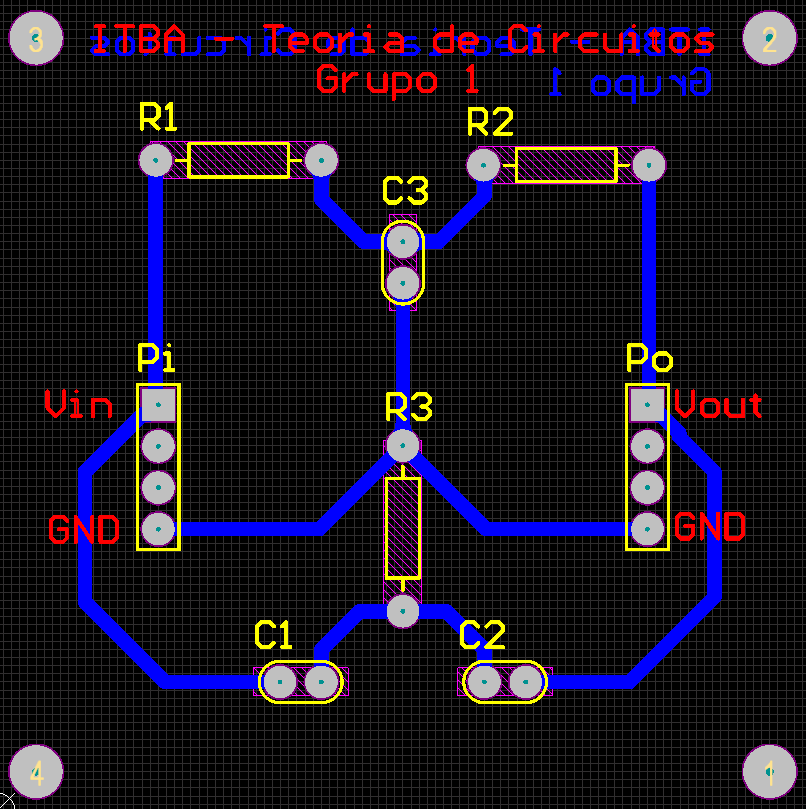
\includegraphics[width=0.7\textwidth]{./EJ1/PCB.png}
        \caption{PCB dise\~nado en el programa Altium Designer.}
        \label{fig: PCB_Altium}
    \end{minipage}\hfill
\end{figure}




\subsubsection{Comparaci\'on de las curvas}
\missingfigure{COMBINATION OF 3 GRAPHS FOR AMPLITUDE BODE}
\todo[inline]{SHORT ANALYSIS OF THE GRAPH}
\missingfigure{COMINATION OF 3 GRAPHS FOR PHASE BODE}
\todo[inline]{SHORT ANALYSIS OF THE GRAPH}
\missingfigure{COMBINATION OF 3 GRAPHS FOR RESPONSE TO HEAVISIDE}
\todo[inline]{SHORT ANALYSIS OF THE GRAPH}

\section{Filtro pasa-bajos pasivo}

\quad \quad En esta secci\'on dise\~naremos y analizaremos el comportamiento de un filtro RC de primer orden pasa-bajos.

\subsection{Dise\~no}
\quad \quad Seg\'un el n\'umero de grupo asignado fijamos la frecuencia de corte del filtro en $16kHz$. Luego calculamos la funci\'on transferencia del mismo obteniendo

\begin{equation}\label{ganancia_2}
H(s) = \frac{1}{sCR+1}
\end{equation}

Donde la frecuencia de corte $f_{0}$ vale

\begin{equation}\label{freccorte_2}
f_{0} = 2\pi CR
\end{equation}

Dado que los valores de ambos componentes son comerciales y estandarizados, seleccionamos un par para los cuales creemos que el error es lo suficientemente peque\~no. As\'i, fijamos $C=10nF$ y $R=1k\Omega$ con lo cual la frecuencia de corte te\'orica es $f_{0}=15915,49Hz$.

\subsection{Se\~nal cuadrada}

\quad \quad Una vez seleccionados los componentes se arm\'o el circuito y se lo someti\'o a una se\~nal cuadrada (cuyo valor medio es nulo) de $10V_{pp}$ a una frecuencia dada de $8kHz$ con la siguiente respuesta medida en osciloscopio.

\begin{figure}[H]
    \centering
    \includegraphics[width=0.9\textwidth]{./EJ2/EJ2_respuesta_a_cuadrada.png}
    \caption{Respuesta a una se\~nal cuadrada}
    \label{fig:rtacuad_2} 
\end{figure}

\quad \quad En la figura \ref{fig:rtacuad_2} se puede observar una forma curva en los flancos ascendentes y descendientes de la respuesta del sistema a la se\~nal cuadrada (curva resaltada en celeste). Esto se debe principalmente a los intervalos de carga y descarga del capacitor, ante la inversi\'on de polaridad en sus bornes, obteniendo ese efecto de $"suavizaci\'on"$. Adem\'as, desde el punto de vista espectral podemos apreciar una atenuaci\'on en los arm\'onicos altos que componen la se\~nal cuadrada, debido a que esta entrada est\'a pasando por un filtro pasa-bajos. Esto tambi\'en contribuye a la distorsi\'on en la forma de la se\~nal.

\subsection{Respuesta en frecuencia}

\quad \quad Para confeccionar la respuesta en frecuencia del filtro se realiz\'o un barrido en frecuencia de la entrada, midiendo a la salida la relaci\'on entre la amplitud respecto a la de la entrada, y la fase. Luego se volcaron esos datos a una hoja de c\'alculo y se obtuvieron dos gr\'aficos que representan cada una de esas caracter\'isticas.

%\begin{figure}[H]
 %   \centering
 %   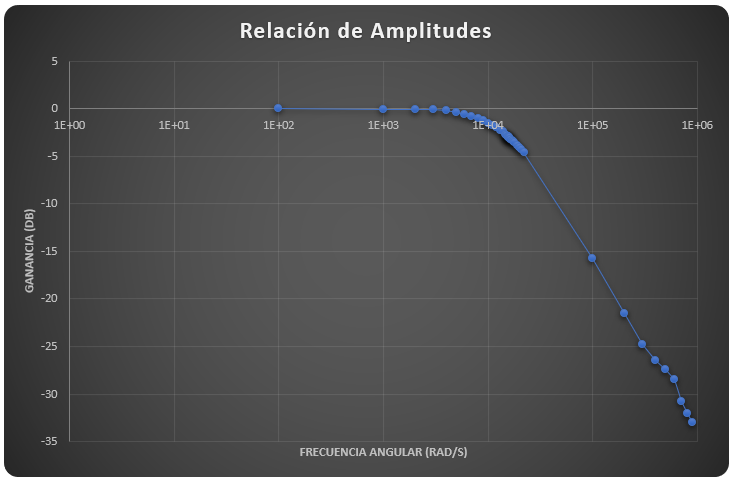
\includegraphics[width=0.9\textwidth]{./EJ2/EJ2_BODE_amp_medido.png}
 %   \caption{Diagrama BODE de amplitud medido}
 %   \label{fig: bode_amp_medido_2} 
%\end{figure}


%\begin{figure}[H]
 %   \centering
 %   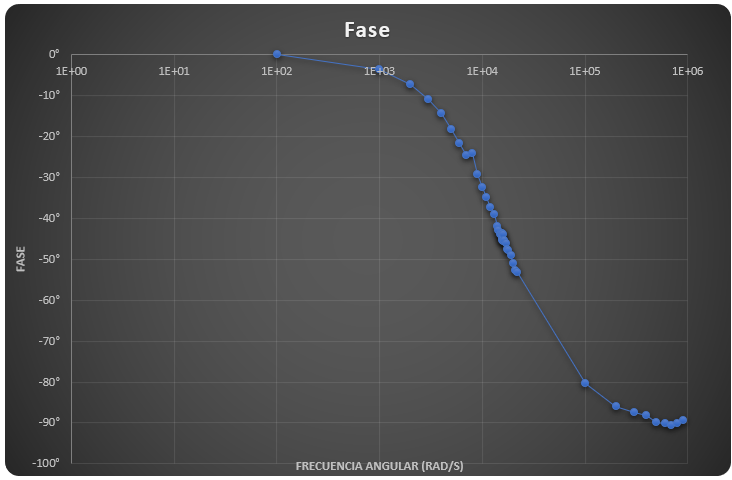
\includegraphics[width=0.9\textwidth]{./EJ2/EJ2_BODE_fase_medido.png}
 %   \caption{Diagrama BODE de fase medido}
 %   \label{fig: bode_fase_medido_2} 
%\end{figure}

\quad \quad La frecuencia de corte $"real"$ del circuito fue obtenida usando el osciloscopio, variando la frecuencia hasta encontrar un desfasaje de $-45^\circ$ en la salida respecto a la entrada. Seg\'un la figura \ref{fig:phase_2}, en este caso $f_{0}=15,57kHz$


\begin{figure}[H]
    \centering
    \includegraphics[width=0.9\textwidth]{./EJ2/EJ2_fase_osc.png}
    \caption{Medici\'on de frecuencia de corte}
    \label{fig:phase_2} 
\end{figure}
\quad \quad Adem\'as, se puede ver que el diagrama de BODE resultante de las mediciones es compatible con el an\'alisis te\'orico sobre el filtro.

\quad \quad Por otro lado, se desarroll\'o en serie de Fourier la se\~nal de entrada con el fin de encontrar las componentes de frecuencia que componen a dicha se\~nal. Usando los coeficientes de Fourier podemos observar la presencia de cada uno de los arm\'onicos (son todos impares), y se superpuso esta informaci\'on con el gr\'afico de amplitud del diagrama de BODE teórico. De esta forma, y calculando la funci\'on transferencia para sucesivos arm\'onicos, se observa que a frecuencias altas la baja amplitud de los arm\'onicos combinado con el bajo valor de la funci\'on transferencia nos permiten despreciar la presencia de dichos arm\'onicos.

\begin{figure}[H]
    \centering
    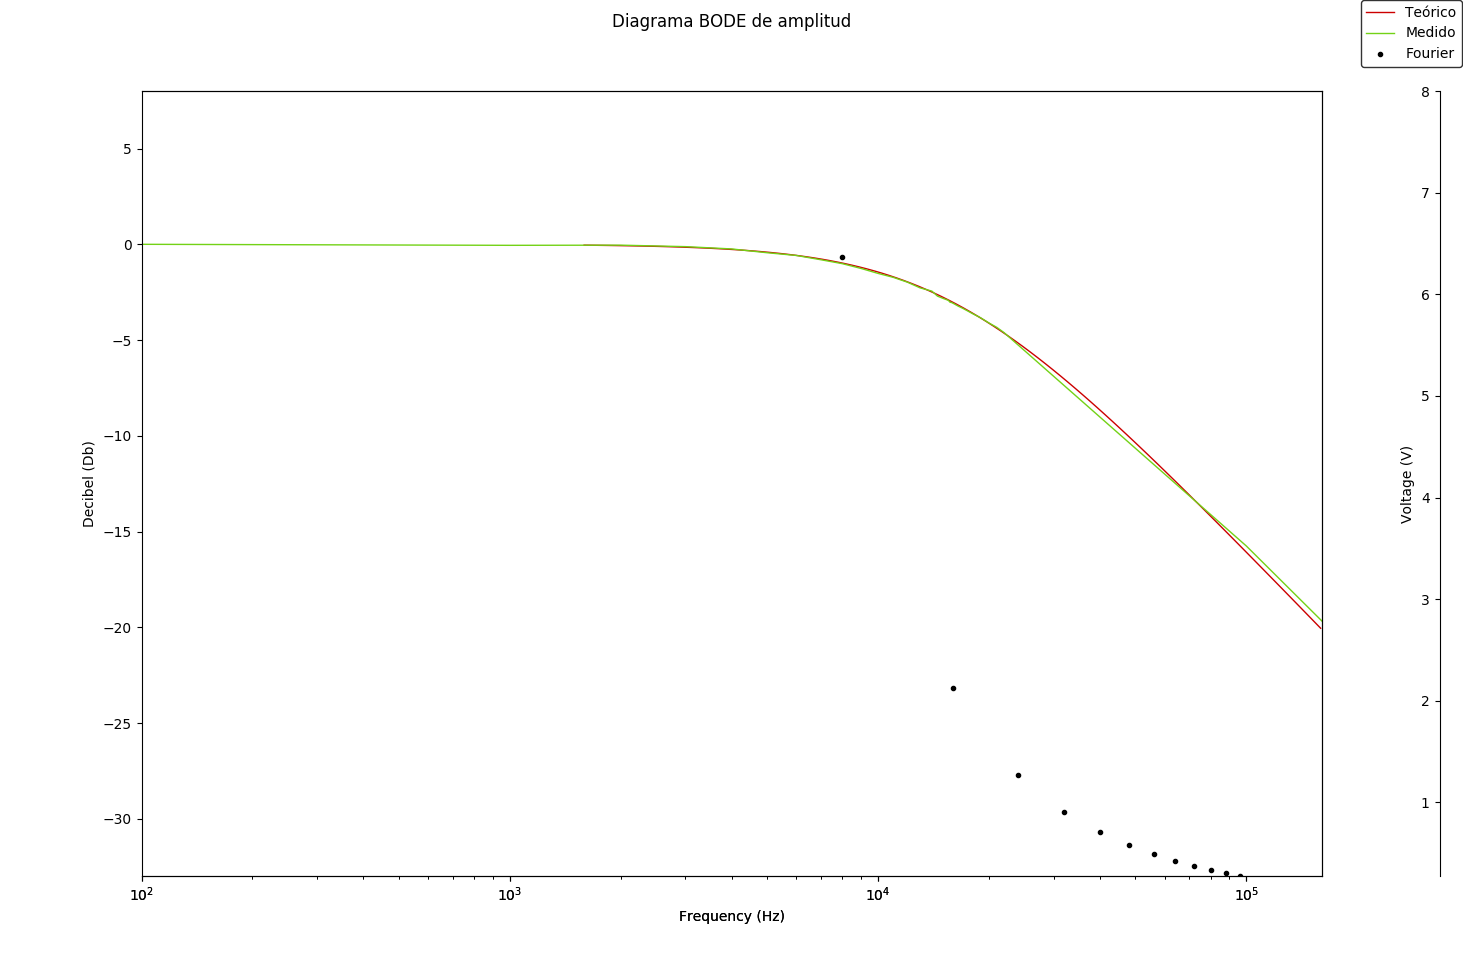
\includegraphics[width=0.9\textwidth]{./EJ2/EJ2_BODE_teorico.png}
    \caption{Diagrama BODE de amplitud te\'orico y medido y amplitud de arm\'onicos de entrada}
    \label{fig:bode_amp_superp_2} 
\end{figure}

\begin{figure}[H]
    \centering
    \includegraphics[width=0.9\textwidth]{./EJ2/EJ2_fase_BODE.png}
    \caption{Diagrama BODE de fase te\'orico y medido}
    \label{fig:bode_phase_superp_2} 
\end{figure}

\subsection{Comportamiento en alta frecuencia}

\quad \quad Si sometemos el circuito a una frecuencia moderadamente alta comparada con la frecuencia de corte del mismo, podemos ver que la funci\'on transferencia tiende a 
\begin{equation}\label{integrador_2}
    H(s)=\frac{1}{s}
\end{equation}

Lo que en transformada de Laplace implicar\'ia la integraci\'on de la se\~nal de entrada. Para comprobar esto forzamos al circuito en la pr\'actica a una frecuencia $f=250kHz$ seg\'un la figura \ref{fig:altafrec_2}. De este gr\'afico podemos resaltar que la se\~nal cuadrada de entrada resulta en una se\~nal de tipo triangular en la salida, confirmando la suposici\'on te\'orica planteada anteriormente.

\begin{figure}[H]
    \centering
    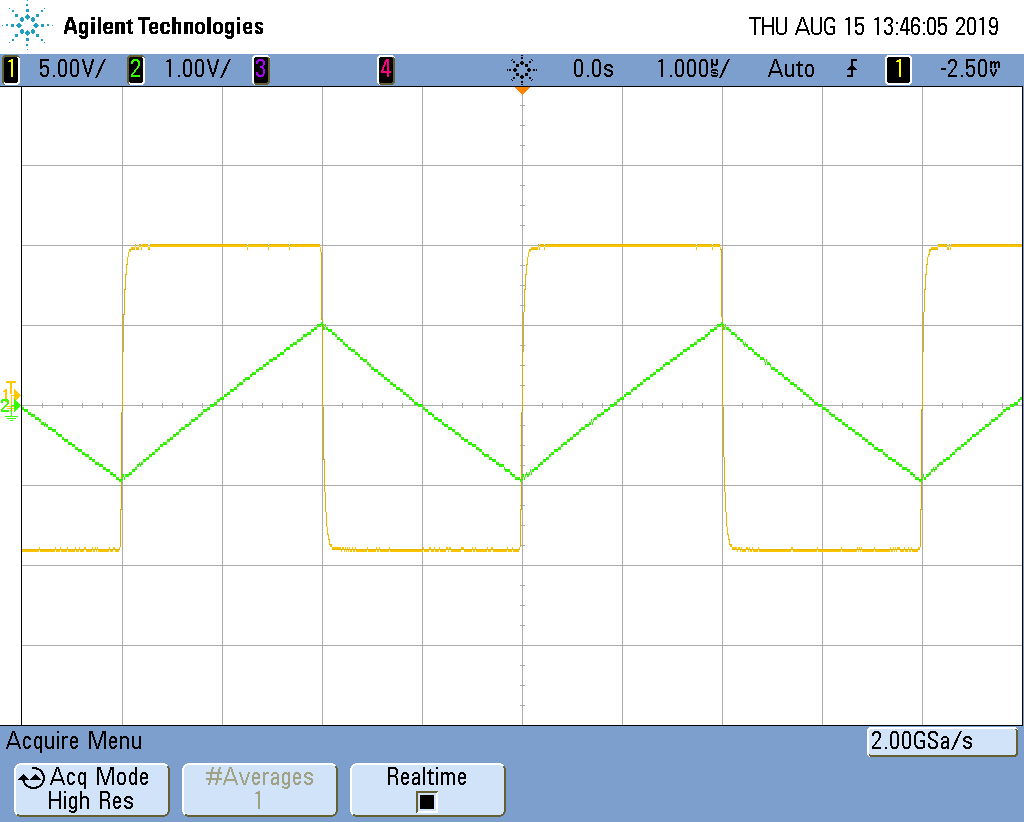
\includegraphics[width=0.9\textwidth]{./EJ2/EJ2_integrador.png}
    \caption{Respuesta a 250kHz}
    \label{fig:altafrec_2} 
\end{figure}

\quad \quad Si ahora probamos una frecuencia mucho mayor (en este caso $10MHz$) observamos una atenuaci\'on de la se\~nal de salida considerable, lo que produce que la salida sea susceptible de ser afectada por el ruido, como se puede ver en la figura \ref{fig:noise_2}.
 
 \begin{figure}[H]
    \centering
    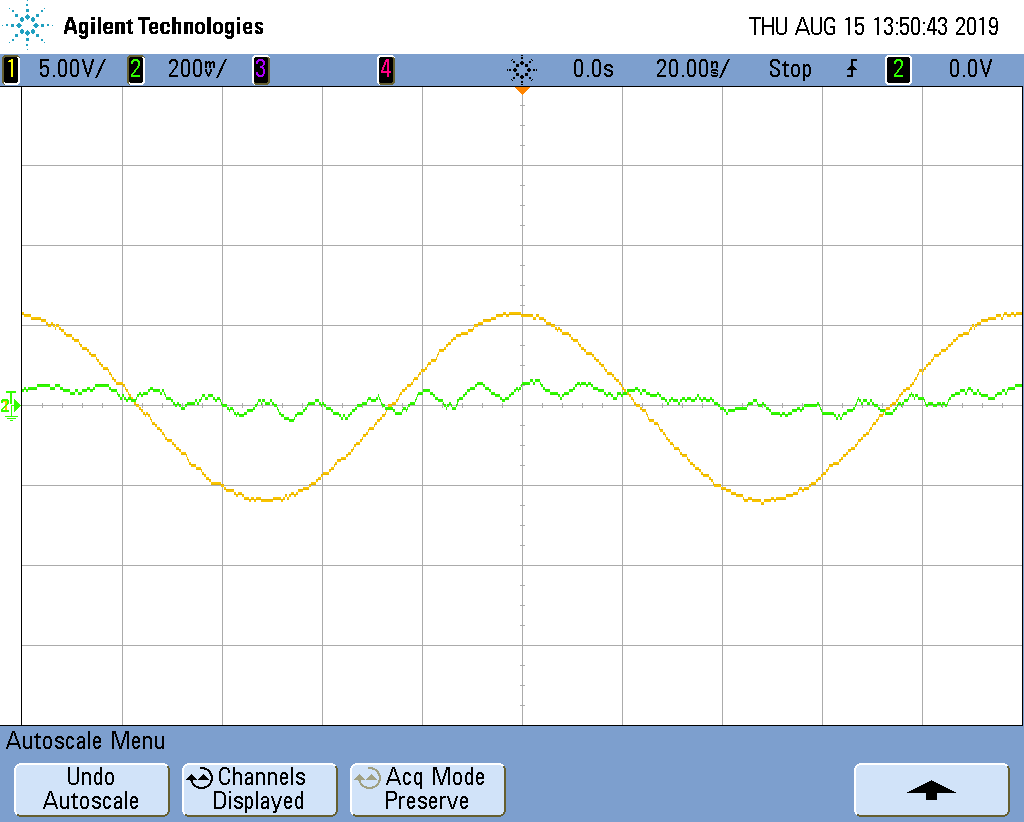
\includegraphics[width=0.9\textwidth]{./EJ2/EJ2_rta_alta_frec.png}
    \caption{Respuesta a 10MHz}
    \label{fig:noise_2}
\end{figure}
 
\subsection{Respuesta a $160Hz$}

\quad \quad Se conect\'o la entrada del circuito a una se\~nal cuadrada de similares caracter\'isticas que la primera, pero esta vez a una frecuencia de $160Hz$. Se midi\'o con osciloscopio la respuesta del circuito y se obtuvo la figura \ref{fig:160hz_2}. En ella podemos observar una atenuaci\'on casi nula de la salida (representada en color celeste) respecto de la entrada, asi como una fase pr\'acticamente nula. Esto se condice con el an\'alisis te\'orico que se puede realizar, dado que el t\'ermino que involucra a la frecuencia en la ecuaci\'on \ref{ganancia_2} se vuelve despreciable, con lo cual la funci\'on transferencia tiende al valor unitario.

\begin{figure}[H]
    \centering
    \includegraphics[width=0.9\textwidth]{./EJ2/EJ2_rta_160hz.png}
    \caption{Respuesta a $160Hz$}
    \label{fig:160hz_2} 
\end{figure}


%\section{Ejercicio 3: Plot-Tool}
\quad \quad En este ejercicio se nos pidi\'o hacer una herramienta para graficar. Los c\'odigos de la misma se encuentran en la carpeta plot-tool entregada en este trabajo pr\'actico y su manual de uso tamb\'en se encuentra dentro de la misma, con el nombre $manual.pdf$. 
%\input{appendix.tex}
%


\end{document}
